% 图 63.4 —— 由 `checks/emit_hand.py` 自动拼出（probe 精测 + prims2 图元分解）
%%
% ⚠ 这是**稿子不是成品**：跑 `checks/checkhand.py 63.4` 看指标 + 看叠合图。
%%
%% ⚠ 待核：
%   · 本图 probe 报出阴影族 1 个 —— **本脚本不生成阴影**（要照原书手写）；prims2 的 strokes 里可能含阴影线，核对时留意别画重
%   · 可疑字形 1 项（空心圈 ⊙ 常被认成字母 o）—— 见文件末
%%
\documentclass[12pt]{standalone}
\usepackage{fontspec}
\setsansfont{Arial}
\newfontfamily\mfallback{DejaVu Sans}
\usepackage{tikz}
\begin{document}
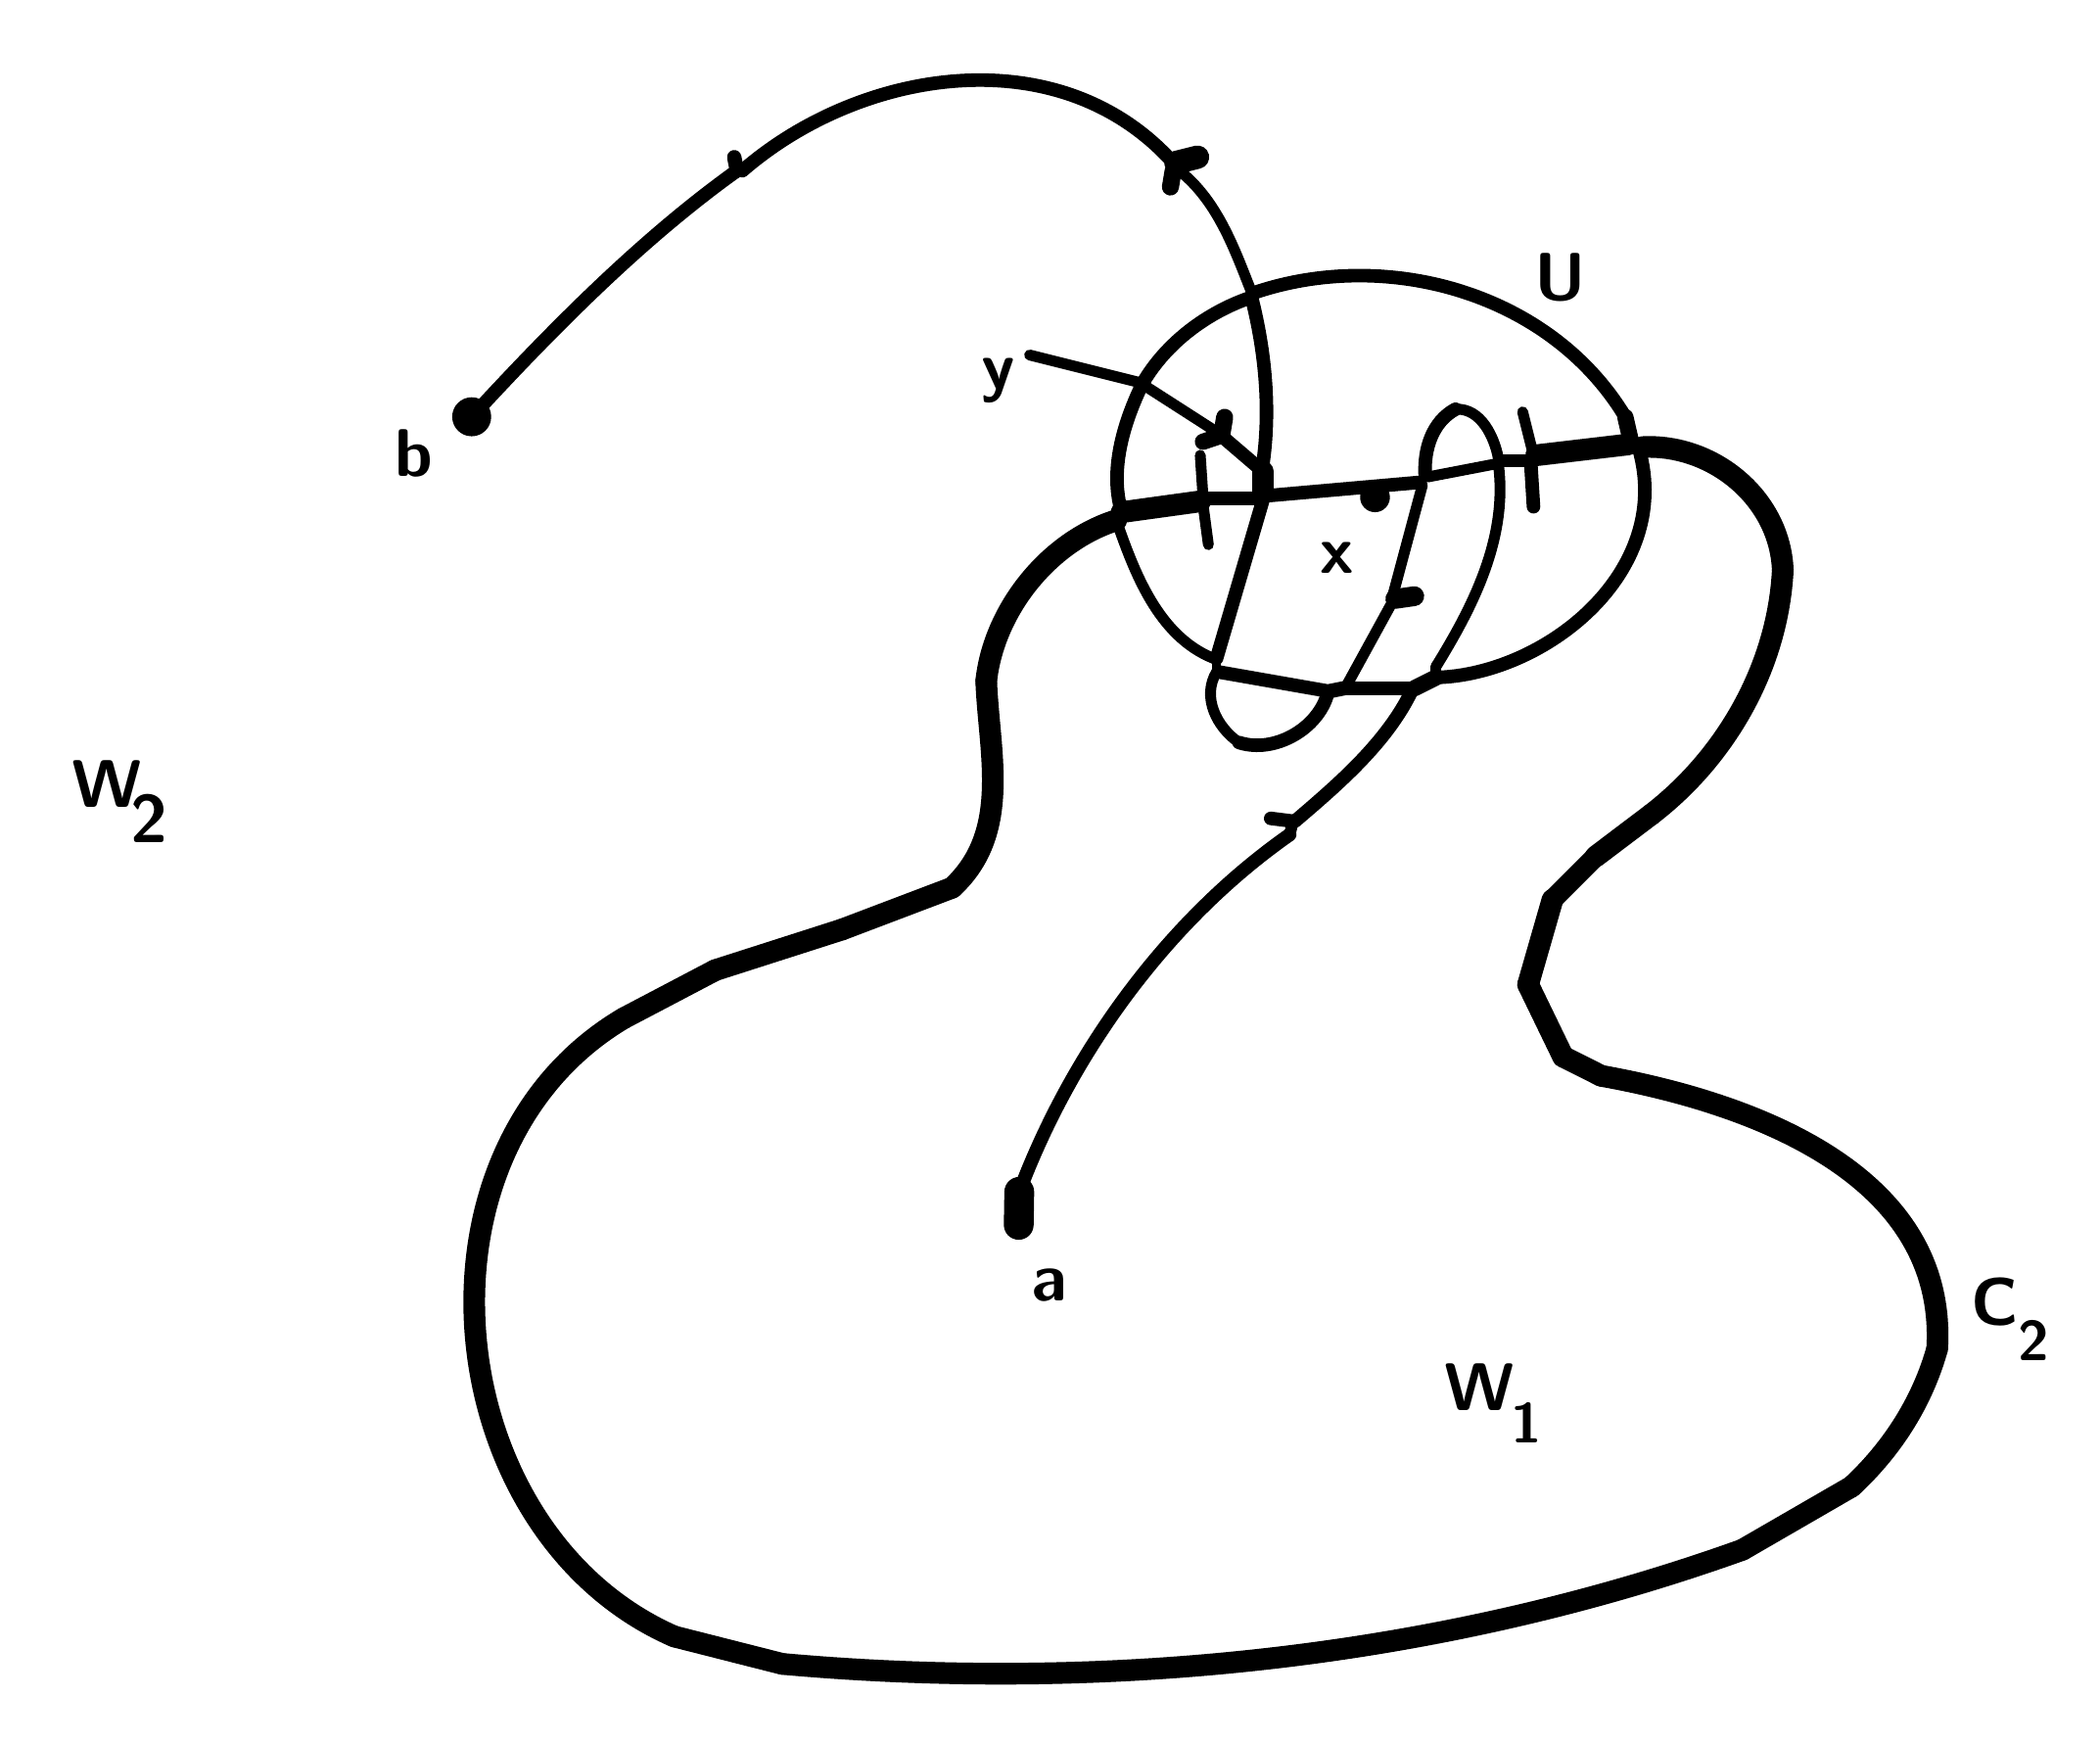
\begin{tikzpicture}[x=1pt, y=-1pt, line width=6.0pt, line cap=round, line join=round]

  %% ════ 填充区（prims2 的 fills）════

  %% ════ 直线段（prims2 的 strokes）════
  \draw[line width=6.0pt] (434.0,153.0) -- (440.0,151.0);
  \draw[line width=4.3pt] (467.0,294.0) -- (466.0,298.0);
  \draw[line width=8.0pt] (591.0,154.0) -- (557.0,158.0);
  \draw[line width=4.0pt] (436.0,191.0) -- (434.0,176.0);
  \draw[line width=5.0pt] (556.0,177.0) -- (555.0,161.0);
  \draw[line width=4.0pt] (433.0,158.0) -- (434.0,173.0);
  \draw[line width=6.0pt] (592.0,153.0) -- (589.9,143.9);
  \draw[line width=8.0pt] (433.0,175.0) -- (404.0,179.0);
  \draw[line width=5.3pt] (486.0,244.0) -- (481.0,245.0);
  \draw[line width=11.0pt] (366.2,429.8) -- (366.0,442.0);
  \draw[line width=4.0pt] (543.0,161.0) -- (517.0,166.0);
  \draw[line width=4.0pt] (520.0,236.0) -- (520.0,240.0);
  \draw[line width=3.0pt] (439.0,234.0) -- (439.0,237.0);
  \draw[line width=4.0pt] (487.0,243.0) -- (504.0,212.0);
  \draw[line width=4.0pt] (410.0,131.0) -- (370.0,121.0);
  \draw[line width=5.0pt] (544.0,160.0) -- (554.0,160.0);
  \draw[line width=4.0pt] (556.0,158.0) -- (552.0,142.0);
  \draw[line width=5.0pt] (480.0,245.0) -- (440.0,238.0);
  \draw[line width=4.0pt] (515.0,169.0) -- (504.0,210.0);
  \draw[line width=8.6pt] (424.0,50.0) -- (432.0,48.0);
  \draw[line width=8.0pt] (456.0,172.0) -- (456.0,164.0);
  \draw[line width=5.0pt] (457.0,173.0) -- (514.0,168.0);
  \draw[line width=7.3pt] (505.0,211.0) -- (512.0,210.0);
  \draw[line width=4.0pt] (440.0,150.0) -- (412.0,132.0);
  \draw[line width=6.3pt] (442.0,144.0) -- (441.0,150.0);
  \draw[line width=5.0pt] (467.0,293.0) -- (459.0,292.0);
  \draw[line width=6.3pt] (422.0,59.0) -- (423.0,53.0);
  \draw[line width=5.3pt] (262.0,53.0) -- (261.0,48.0);
  \draw[line width=8.0pt] (599.4,290.6) -- (578.9,306.1);
  \draw[line width=7.5pt] (578.9,306.1) -- (563.0,322.0);
  \draw[line width=8.0pt] (563.0,322.0) -- (554.0,353.3);
  \draw[line width=8.0pt] (554.0,353.3) -- (566.9,379.9);
  \draw[line width=8.0pt] (566.9,379.9) -- (581.0,387.0);
  \draw[line width=8.0pt] (673.4,538.6) -- (633.1,561.9);
  \draw[line width=8.0pt] (278.7,604.0) -- (238.9,593.9);
  \draw[line width=8.0pt] (220.3,365.7) -- (254.0,348.0);
  \draw[line width=8.0pt] (254.0,348.0) -- (300.8,333.0);
  \draw[line width=8.0pt] (300.8,333.0) -- (341.4,317.6);
  \draw[line width=3.8pt] (404.0,179.0) -- (402.0,182.0);
  \draw[line width=6.0pt] (520.0,240.0) -- (512.0,244.0);
  \draw[line width=5.0pt] (510.0,244.0) -- (487.0,244.0);
  \draw[line width=5.0pt] (439.0,233.0) -- (456.0,175.0);
  \draw[line width=5.0pt] (435.0,174.0) -- (455.0,174.0);
  \draw[line width=5.0pt] (441.0,151.0) -- (455.0,163.0);

  %% ════ 曲线（prims2 的 curves —— 三段式，坐标同为 (y,x)）════
  \draw[line width=4.0pt] (424.0,52.0) .. controls (439.2,63.2) and (445.6,81.9) .. (452.0,98.0);
  \draw[line width=5.0pt] (589.9,143.9) .. controls (562.3,98.0) and (501.9,81.4) .. (453.0,98.0);
  \draw[line width=4.0pt] (438.0,233.0) .. controls (417.3,224.8) and (408.5,200.6) .. (402.0,182.0);
  \draw[line width=5.0pt] (163.0,145.0) .. controls (193.0,112.4) and (226.2,78.6) .. (262.0,53.0);
  \draw[line width=5.0pt] (466.0,298.0) .. controls (420.3,330.0) and (385.2,379.2) .. (366.2,429.8);
  \draw[line width=4.0pt] (543.0,161.0) .. controls (546.7,188.3) and (533.8,213.6) .. (520.0,236.0);
  \draw[line width=4.0pt] (439.0,238.0) .. controls (433.5,247.2) and (439.0,258.3) .. (447.3,264.0);
  \draw[line width=5.0pt] (447.3,264.0) .. controls (460.4,268.2) and (476.5,258.9) .. (480.0,246.0);
  \draw[line width=4.0pt] (543.0,159.0) .. controls (541.6,151.5) and (536.7,140.5) .. (527.2,141.0);
  \draw[line width=5.0pt] (527.2,141.0) .. controls (518.6,145.7) and (515.6,155.6) .. (516.0,165.0);
  \draw[line width=8.0pt] (596.0,155.0) .. controls (622.2,153.5) and (647.0,173.9) .. (648.0,200.4);
  \draw[line width=8.0pt] (648.0,200.4) .. controls (646.2,235.6) and (627.4,269.1) .. (599.4,290.6);
  \draw[line width=8.0pt] (581.0,387.0) .. controls (632.5,396.2) and (708.9,421.3) .. (705.0,487.7);
  \draw[line width=8.0pt] (705.0,487.7) .. controls (699.6,506.9) and (688.8,524.3) .. (673.4,538.6);
  \draw[line width=8.0pt] (633.1,561.9) .. controls (523.3,601.3) and (400.2,614.9) .. (278.7,604.0);
  \draw[line width=8.0pt] (238.9,593.9) .. controls (152.0,556.0) and (136.7,415.2) .. (220.3,365.7);
  \draw[line width=8.0pt] (341.4,317.6) .. controls (363.5,297.2) and (355.0,267.7) .. (354.0,241.3);
  \draw[line width=8.0pt] (354.0,241.3) .. controls (356.8,215.4) and (376.7,190.0) .. (402.0,182.0);
  \draw[line width=5.0pt] (264.0,53.0) .. controls (307.3,15.4) and (380.8,3.1) .. (423.0,50.0);
  \draw[line width=5.0pt] (404.0,179.0) .. controls (399.5,163.8) and (404.5,146.8) .. (411.0,133.0);
  \draw[line width=5.0pt] (412.0,131.0) .. controls (420.6,116.4) and (435.5,105.4) .. (451.0,100.0);
  \draw[line width=5.0pt] (452.0,100.0) .. controls (457.0,119.8) and (459.1,141.4) .. (456.0,162.0);
  \draw[line width=5.0pt] (520.0,240.0) .. controls (560.2,239.0) and (607.7,201.3) .. (595.0,156.0);
  \draw[line width=5.0pt] (511.0,245.0) .. controls (501.9,263.9) and (484.2,279.2) .. (468.0,293.0);

  %% ════ 实心点 ════
  \fill (164.1,143.8) circle (7.2);
  \fill (497.5,173.5) circle (5.5);

  %% ════ 标签（probe 直接给的 \node 行）════
  %% ⚠ 全部补了 fill=white：文字在最上层，否则与曲线交叉干扰
     \node[anchor=center,inner sep=0pt,fill=white,font=\fontsize{29.6}{37.0}\selectfont] at (566.0,92.2) {\textsf{\textbf{\textit{U}}}};   % box(556,80,20,22)
     \node[anchor=center,inner sep=0pt,fill=white,font=\fontsize{29.8}{37.3}\selectfont] at (358.7,130.2) {\textsf{\textbf{\textit{y}}}};   % box(350,117,17,23)
     \node[anchor=center,inner sep=0pt,fill=white,font=\fontsize{30.0}{37.5}\selectfont] at (142.8,157.2) {\textsf{\textbf{\textit{b}}}};   % box(133,145,17,22)
     \node[anchor=center,inner sep=0pt,fill=white,font=\fontsize{29.2}{36.5}\selectfont] at (483.5,195.9) {\textsf{\textbf{\textit{x}}}};   % box(474,186,17,16)
     \node[anchor=center,inner sep=0pt,fill=white,font=\fontsize{28.0}{35.0}\selectfont] at (29.7,279.4) {\textsf{\textbf{\textit{W}}}};   % box(17,268,25,21)
     \node[anchor=center,inner sep=0pt,fill=white,font=\fontsize{22.9}{28.7}\selectfont] at (45.1,292.4) {\textsf{\textbf{2}}};   % box(39,284,11,16)
     \node[anchor=center,inner sep=0pt,fill=white,font=\fontsize{30.0}{37.6}\selectfont] at (377.5,464.5) {\textsf{\textbf{\textit{a}}}};   % box(369,455,15,16)
     \node[anchor=center,inner sep=0pt,fill=white,font=\fontsize{32.9}{41.2}\selectfont] at (726.3,470.3) {\textsf{\textbf{\textit{C}}}};   % box(715,458,21,24)
     \node[anchor=center,inner sep=0pt,fill=white,font=\fontsize{22.5}{28.2}\selectfont] at (740.6,484.9) {\textsf{\textbf{2}}};   % box(735,476,10,17)
     \node[anchor=center,inner sep=0pt,fill=white,font=\fontsize{29.2}{36.6}\selectfont] at (536.2,502.0) {\textsf{\textbf{\textit{W}}}};   % box(523,490,26,22)
     \node[anchor=center,inner sep=0pt,fill=white,font=\fontsize{20.6}{25.7}\selectfont] at (553.4,515.3) {\textsf{\textbf{1}}};   % box(548,507,6,16)

  % 钉死画布：否则超出的图元/控制点会把页面撑大，1:1 回比就失准
  \pgfresetboundingbox
  \path[use as bounding box] (0,0) rectangle (755,623);
\end{tikzpicture}
\end{document}

% ⚠ 待核清单（probe 拿不准，人眼过一遍）：
%   · 未识别/跳过：⑤ 跳过/未识别的字形
